\documentclass[a4paper,12pt]{article}
\usepackage{WSEIRap} 
\usepackage{pgf-umlcd}
\renewcommand{\titleLab}{Documenting Tasks from Laboratory Exercises}
\renewcommand{\Author}{Your Name}
\renewcommand{\Students}{~}
\renewcommand{\lab}{Zarządznie projektami IT}
\renewcommand{\groupLab}{Gr-1}
\renewcommand{\Date}{1-10-2024}
\renewcommand{\Rodzaj}{Raport}

\begin{document}
\RapPage
Lorem Ipsum is simply dummy text of the printing and typesetting industry. Lorem Ipsum has been the industry's standard dummy text ever since the 1500s, when an unknown printer took a galley of type and scrambled it to make a type specimen book. It has survived not only five centuries, but also the leap into electronic typesetting, remaining essentially unchanged. 

\section{Basic class of uml}
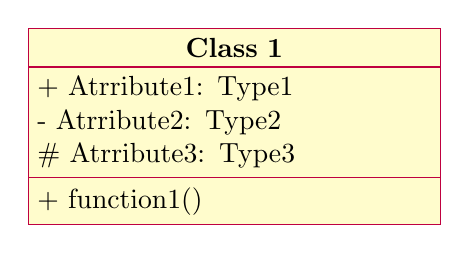
\begin{tikzpicture}
\begin{class}{Class 1}{0,0}
\attribute{+ Atrribute1: Type1}
\attribute{- Atrribute2: Type2}
\attribute{\# Atrribute3: Type3}
\operation{+ function1()}
\end{class}
\end{tikzpicture}

\begin{enumerate}
\item Item 1
\begin{enumerate}
\item Item 1 \textit{italic  text}
\item Item 2 \textbf{Our text}
\end{enumerate}
\item Item 2
\end{enumerate}
\subsection{subsection}
\begin{itemize}
\item Item 1
\item Item 2
\end{itemize}
\section{Title 2}
It was popularised in the 1960s with the release of Letraset sheets containing Lorem Ipsum passages, and more recently with desktop publishing software like Aldus PageMaker including versions of Lorem Ipsum.
\begin{equation}
E=mC^2
\end{equation}
  \begin{figure}
  \centering
  \begin{tikzpicture}[node distance=2.0cm, every node/.style={text width=3cm, align=center, rounded corners, minimum height=0.5cm}]
    \node (po) [fill=red!50] {Product Owner};
    \node (sm) [fill=blue!50, right=of po] {Scrum Master};
    \node (dev) [fill=green!50, below=of sm] {Developer};
    \node (qa) [fill=yellow!50, below left=of po] {Tester / QA};
    \node (devops) [fill=orange!50, below=of dev] {DevOps};
    \draw[<->, thick] (dev) -- (devops) node[midway, right] {Możliwe};
    \draw[<->, thick] (po) -- (sm) node[midway, above] {Nie zalecane};
    \draw[<->, thick] (po) -- (dev) node[midway, left] {Nie zalecane};
    \draw[<->, thick] (sm) -- (dev) node[midway, right] {Możliwe};
    \draw[<->, thick] (po) -- (qa) node[midway, above] {Nie zalecane};
  \end{tikzpicture}
\caption{Podpis rysunku}
\end{figure}
\begin{figure}
        \begin{ganttchart}[hgrid, vgrid, bar height=0.7,
            bar/.style={fill=blue!50},
            bar label font=\small,
            x unit=0.75cm, y unit chart=0.6cm]{1}{5}
            
            \gantttitle{Plan wykładów}{5} \\
            \gantttitlelist{1,...,5}{1} \\
            
            \ganttbar[bar/.style={fill=green!50}]{Wprowadzenie do zarządzania projektami IT}{1}{1} \\
            \ganttbar[bar/.style={fill=orange!50}]{Metodyki zarządzania projektami IT}{2}{2} \\
            \ganttbar[bar/.style={fill=blue!50}]{Planowanie projektu IT}{3}{3} \\
            \ganttbar[bar/.style={fill=red!50}]{Zarządzanie zespołem i ryzykiem}{4}{4} \\
            \ganttbar[bar/.style={fill=purple!50}]{Monitorowanie i zamykanie projektu}{5}{5} 
        \end{ganttchart}
\caption{Przykład wykresu Gantta}
\end{figure}

\section{Dlaczego dokumentacja musi być staranna?}

\textbf{Dokumentacja techniczna jest fundamentem efektywnego zarządzania projektem. 
Jeśli jest nieczytelna, projekt traci na jakości i efektywności.}

\begin{itemize}
    \item \textbf{Jednolity styl} -- spójność ułatwia zrozumienie i szybkie odnajdywanie informacji.
    \item \textbf{Zgodność z umownymi symbolami} -- stosowanie standardów (np. UML, BPMN) zapewnia uniwersalność i łatwość interpretacji.
    \item \textbf{Czytelność} -- dobrze sformatowane diagramy, akapity i nagłówki pomagają w szybkim przyswajaniu treści.
    \item \textbf{Unikanie chaosu} -- brak konsekwencji w nazewnictwie, nieczytelne schematy i błędne oznaczenia prowadzą do błędów w projekcie.
\end{itemize}

\subsection{Przykład źle przygotowanej dokumentacji}

\begin{figure}[ht]
    \centering
    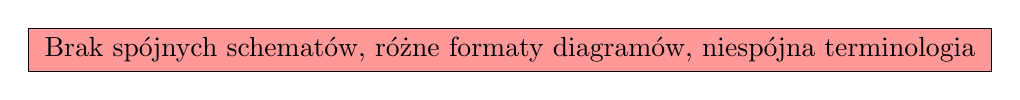
\begin{tikzpicture}
        \node[draw, fill=red!40, text width=12cm, align=center] 
            {Brak spójnych schematów, różne formaty diagramów, niespójna terminologia};
    \end{tikzpicture}
    \caption{Schemat źle przygotowanej dokumentacji}
\end{figure}

\vspace{0.5cm}

\textbf{Konsekwencje:}
\begin{itemize}
    \item Zwiększone ryzyko błędów.
    \item Problemy z wdrażaniem nowych członków zespołu.
    \item Trudności w utrzymaniu systemu.
\end{itemize}

\subsection{Przykład dobrze przygotowanej dokumentacji}

\begin{figure}[ht]
    \centering
    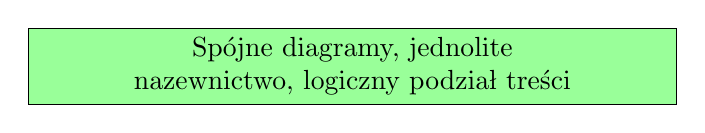
\begin{tikzpicture}
        \node[draw, fill=green!40, text width=8cm, align=center]
            {Spójne diagramy, jednolite nazewnictwo, logiczny podział treści};
    \end{tikzpicture}
    \caption{Schemat dobrze przygotowanej dokumentacji}
\end{figure}

\vspace{0.5cm}

\textbf{Korzyści:}
\begin{itemize}
    \item Szybsze zrozumienie systemu przez nowych członków zespołu.
    \item Ułatwione wdrożenie i rozwój oprogramowania.
    \item Redukcja błędów i problemów komunikacyjnych.
\end{itemize}

\textbf{Dokumentacja powinna być:}
\begin{itemize}
    \item Spójna i jednolita w stylu.
    \item Zgodna z umownymi symbolami.
    \item Czytelnie i przejrzyście sformatowana.
    \item Praktyczna i dostosowana do odbiorców.
\end{itemize}

\end{document}